%%%%%%%%%%%%%%%%%%%%%%%%%%%%%%%%%%%%%%%%%%%%%%%%%%%%%%%%%%%%%%%%%%%%%%%%%%%%%%%%
\section{Supplementary materials}
%%%%%%%%%%%%%%%%%%%%%%%%%%%%%%%%%%%%%%%%%%%%%%%%%%%%%%%%%%%%%%%%%%%%%%%%%%%%%%%%

\begin{figure}[!htbp]
  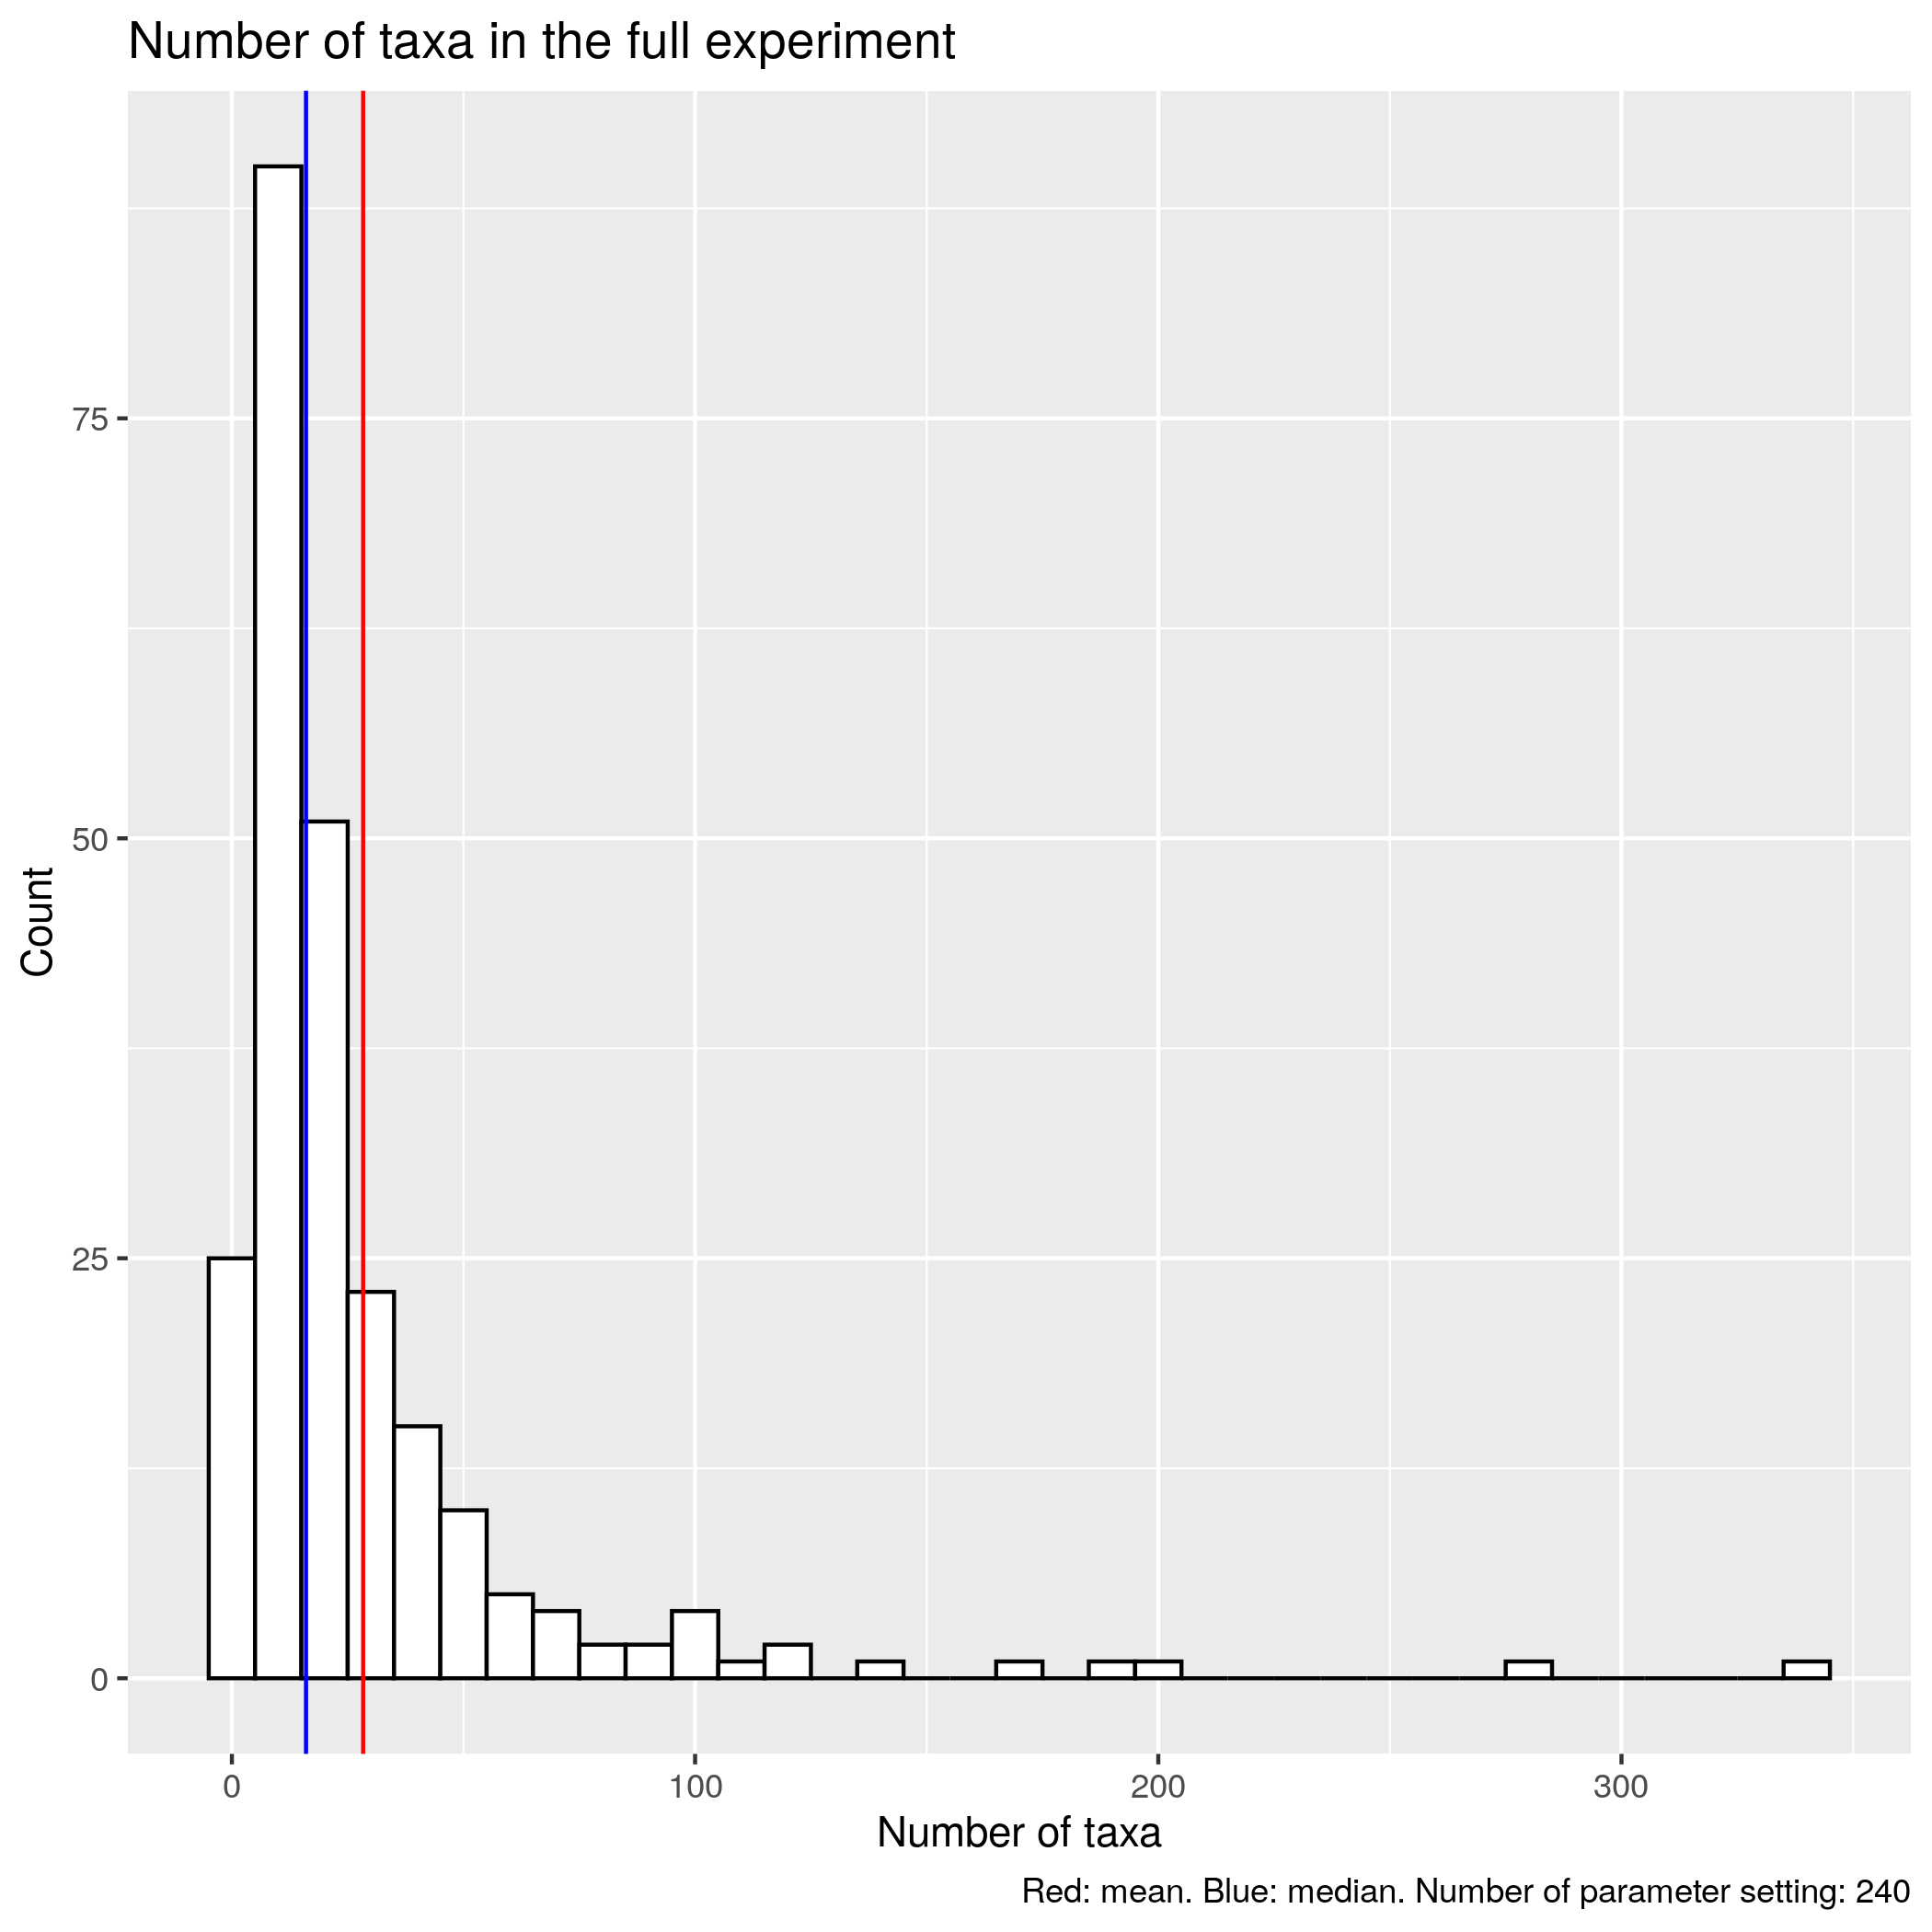
\includegraphics[width=\textwidth]{20190905_fig_n_taxa.png}
  \label{fig:n_taxa}
\end{figure}

\begin{figure}[!htbp]
  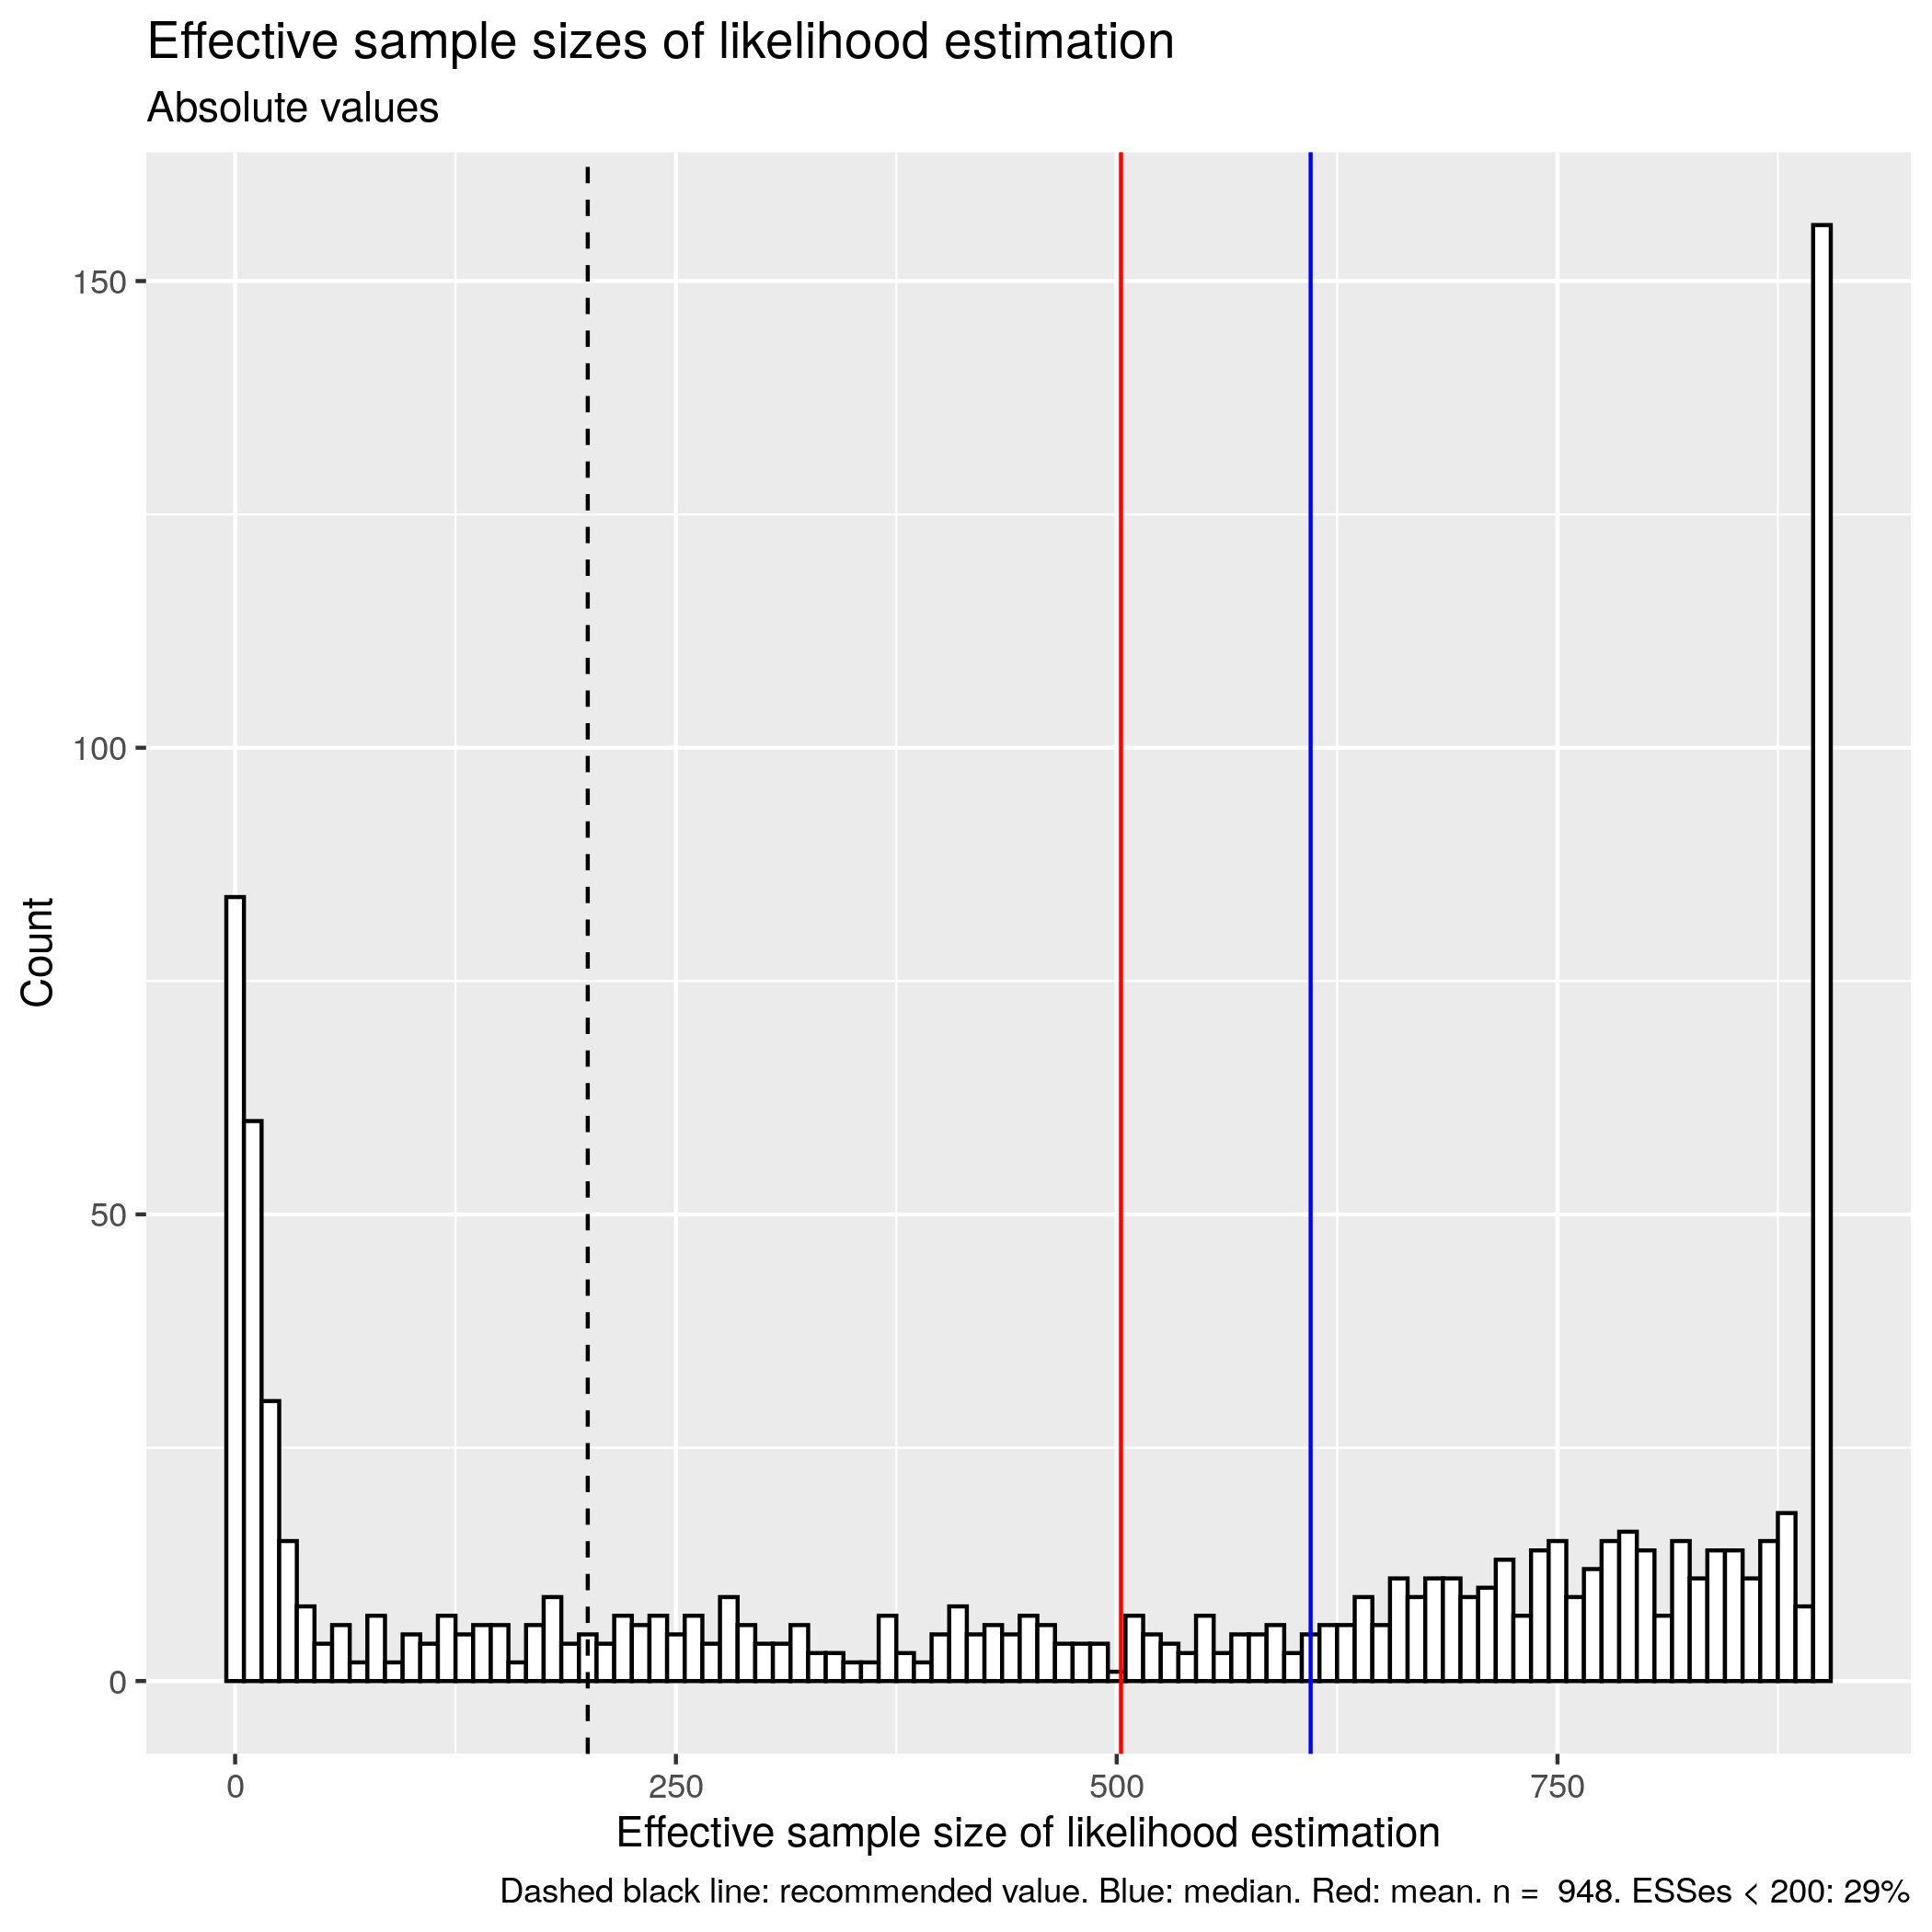
\includegraphics[width=\textwidth]{20190905_fig_esses.png}
  \label{fig:esses}
\end{figure}

\begin{figure}[!htbp]
  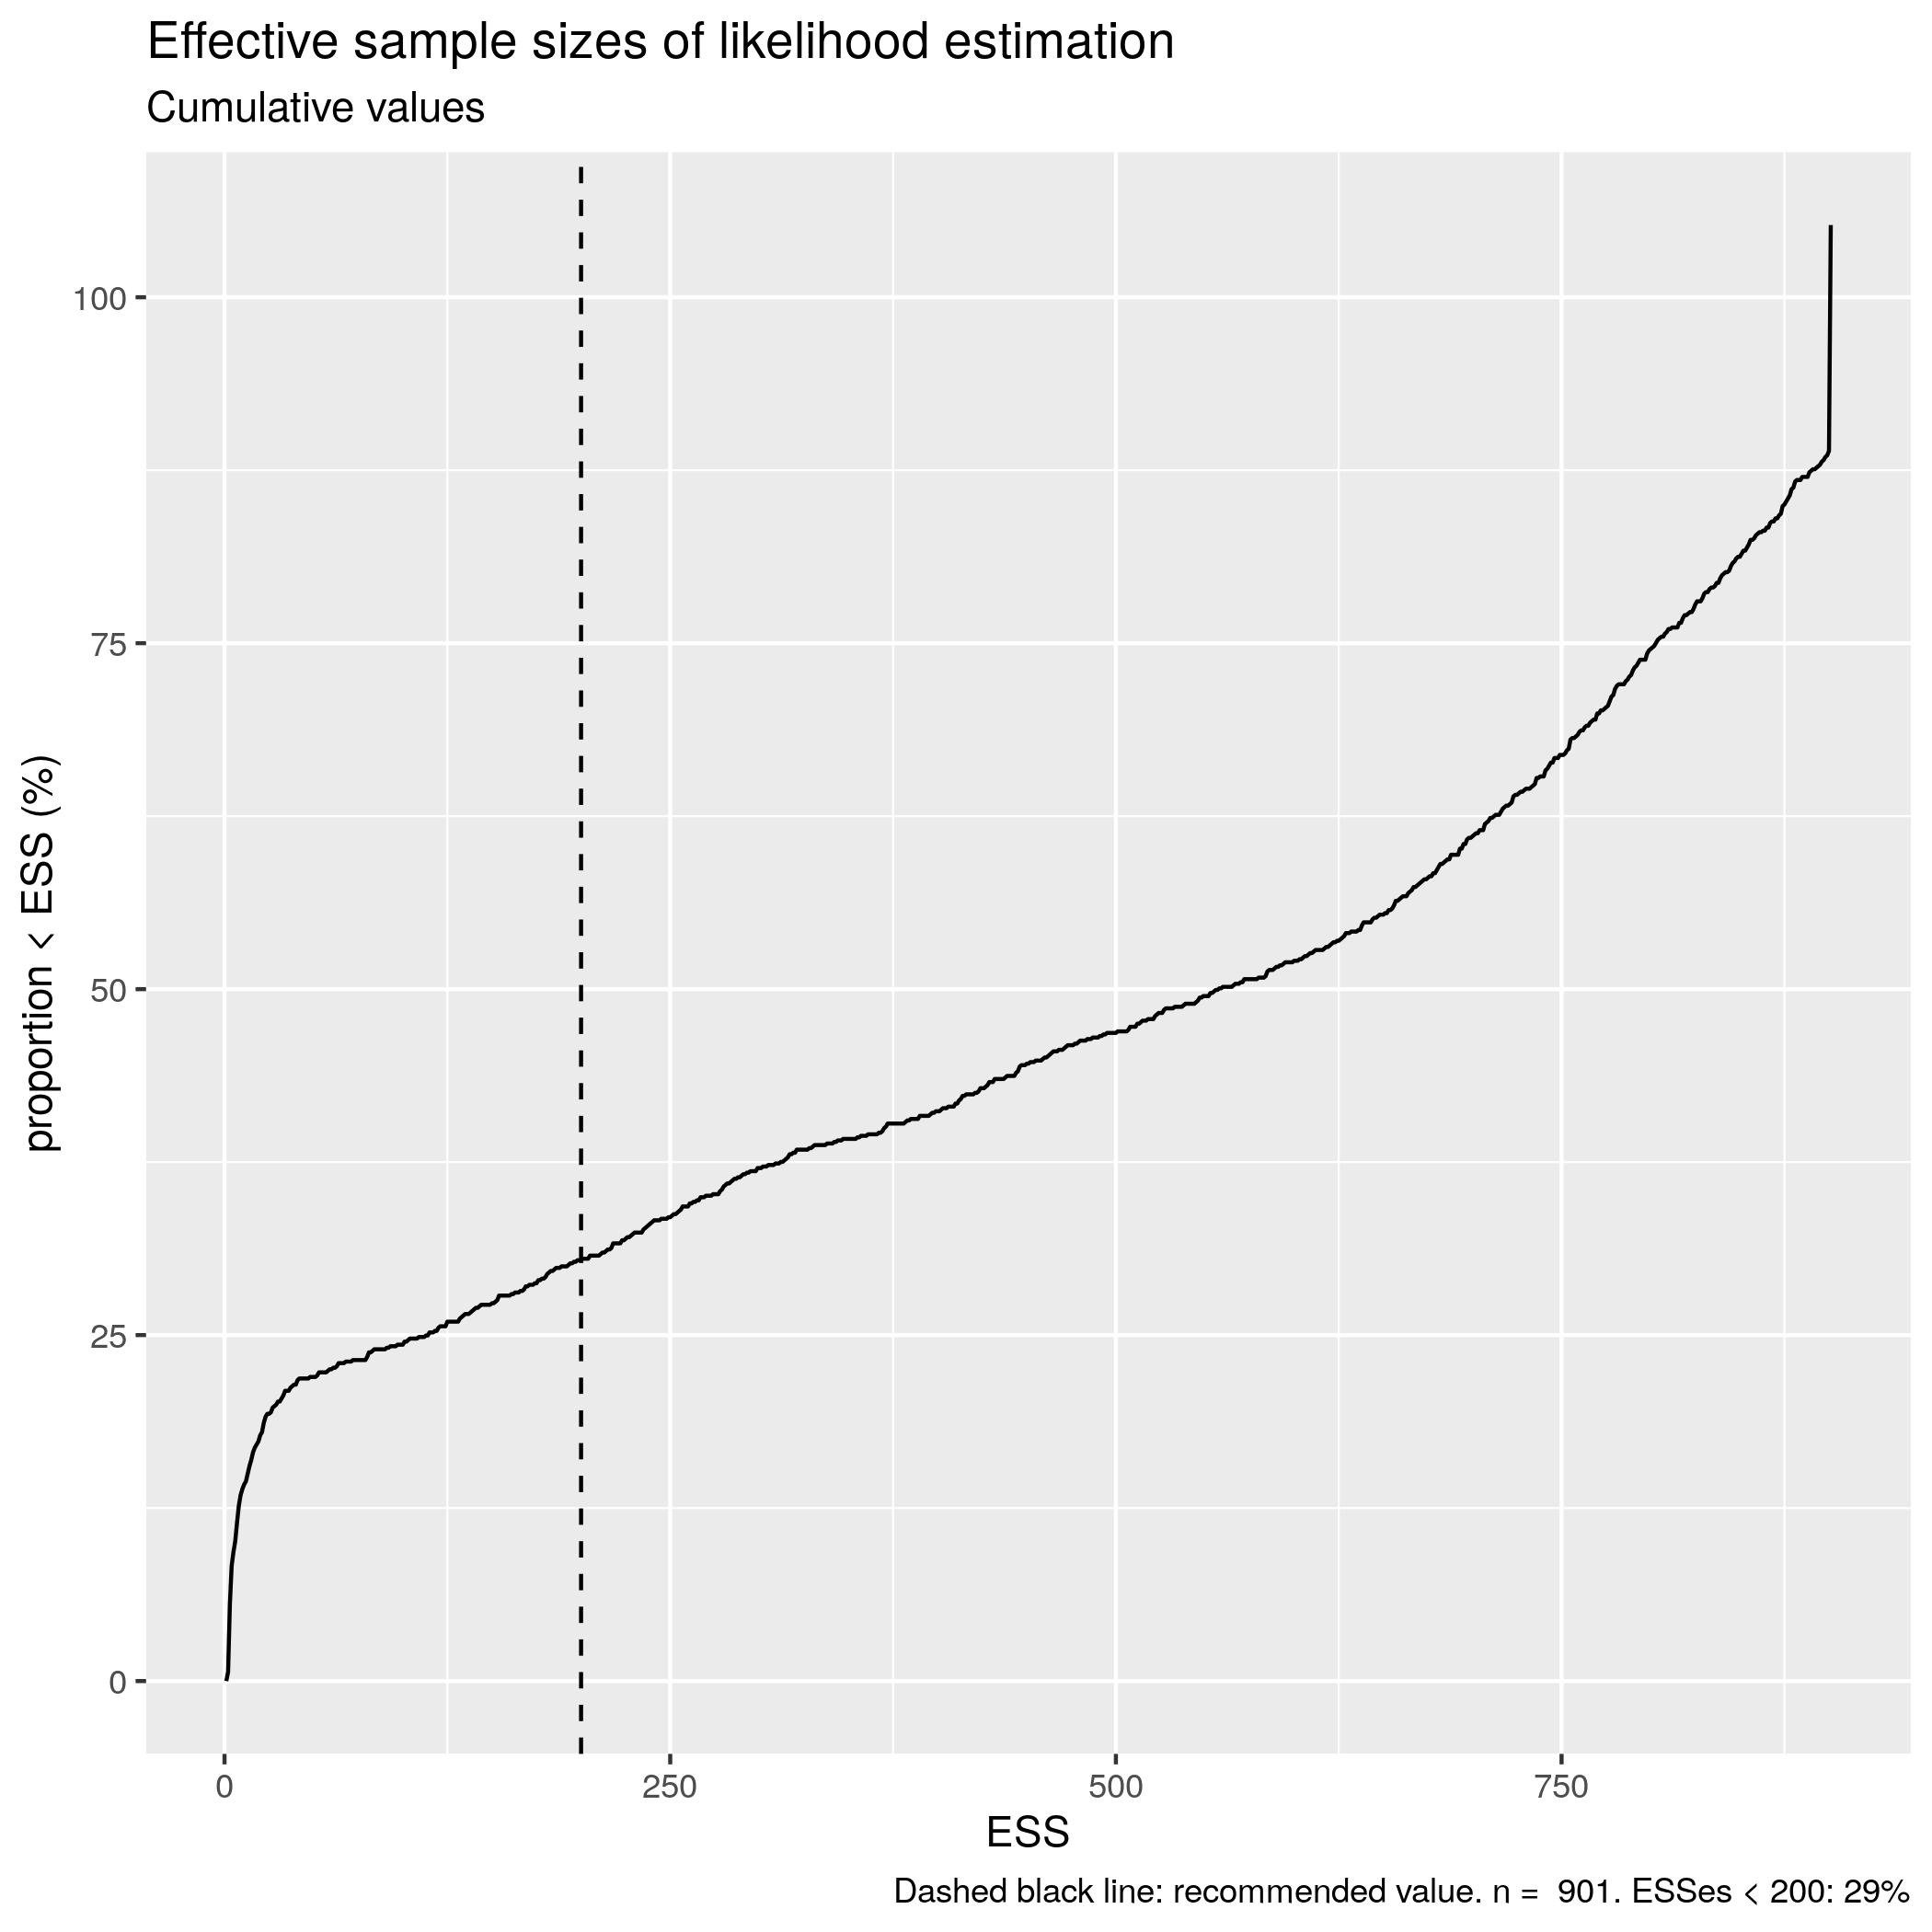
\includegraphics[width=\textwidth]{20190905_fig_esses_cumulative.png}
  \label{fig:esses_cumulative}
  \caption{\richel{n = 901 is something sloppy: the maximum ESS is 901. Next
    to that, the number of ESSes is approx 946}}
\end{figure}




